\documentclass[lang=en]{sjtuarticle}
\title{A Survey of TEE and its Applications}
\author{Log Creative}
\sjtusetup{info/date={2024-06-02}}
\graphicspath{{figs/}}
\usepackage[style=ieee]{biblatex}
\addbibresource{ref.bib}
\usepackage[colorlinks]{hyperref}

\ExplSyntaxOn
\cs_set_eq:NN \circlednumber \__sjtu_footnote_number:N
\ExplSyntaxOff

\begin{document}
\maketitle

\tableofcontents*

\section{SOTA of TEE}

TEE (Trusted Execution Environments) provides an isolated environment (called secure enclave) that safeguards processed data by
encrypting the incoming and outgoing data. Furthermore, TEE provides mechanisms to ensure the
computation is correctly executed with an integrity guarantee. More importantly, TEE protects the
data and computation against any potentially malicious entity residing in the system (including the
kernel, hypervisor, etc.) \cite{li2023survey}.

The current state-of-the-art (SOTA) of TEE are Intel TDX, AMD SEV-SNP, Arm CCA, and RISK-V-based Penglai.

\subsection{Intel TDX}

Intel TDX (Trust Domain Extensions) \cite{tdx} is Intel's newest confidential computing technology, shown in Figure \ref{fig:tdx}. This hardware-based trusted execution environment (TEE) facilitates the deployment of trust domains (TD), which are hardware-isolated virtual machines (VM) designed to protect sensitive data and applications from unauthorized access. The key features are as follows:

\begin{figure}[h]
    \centering
    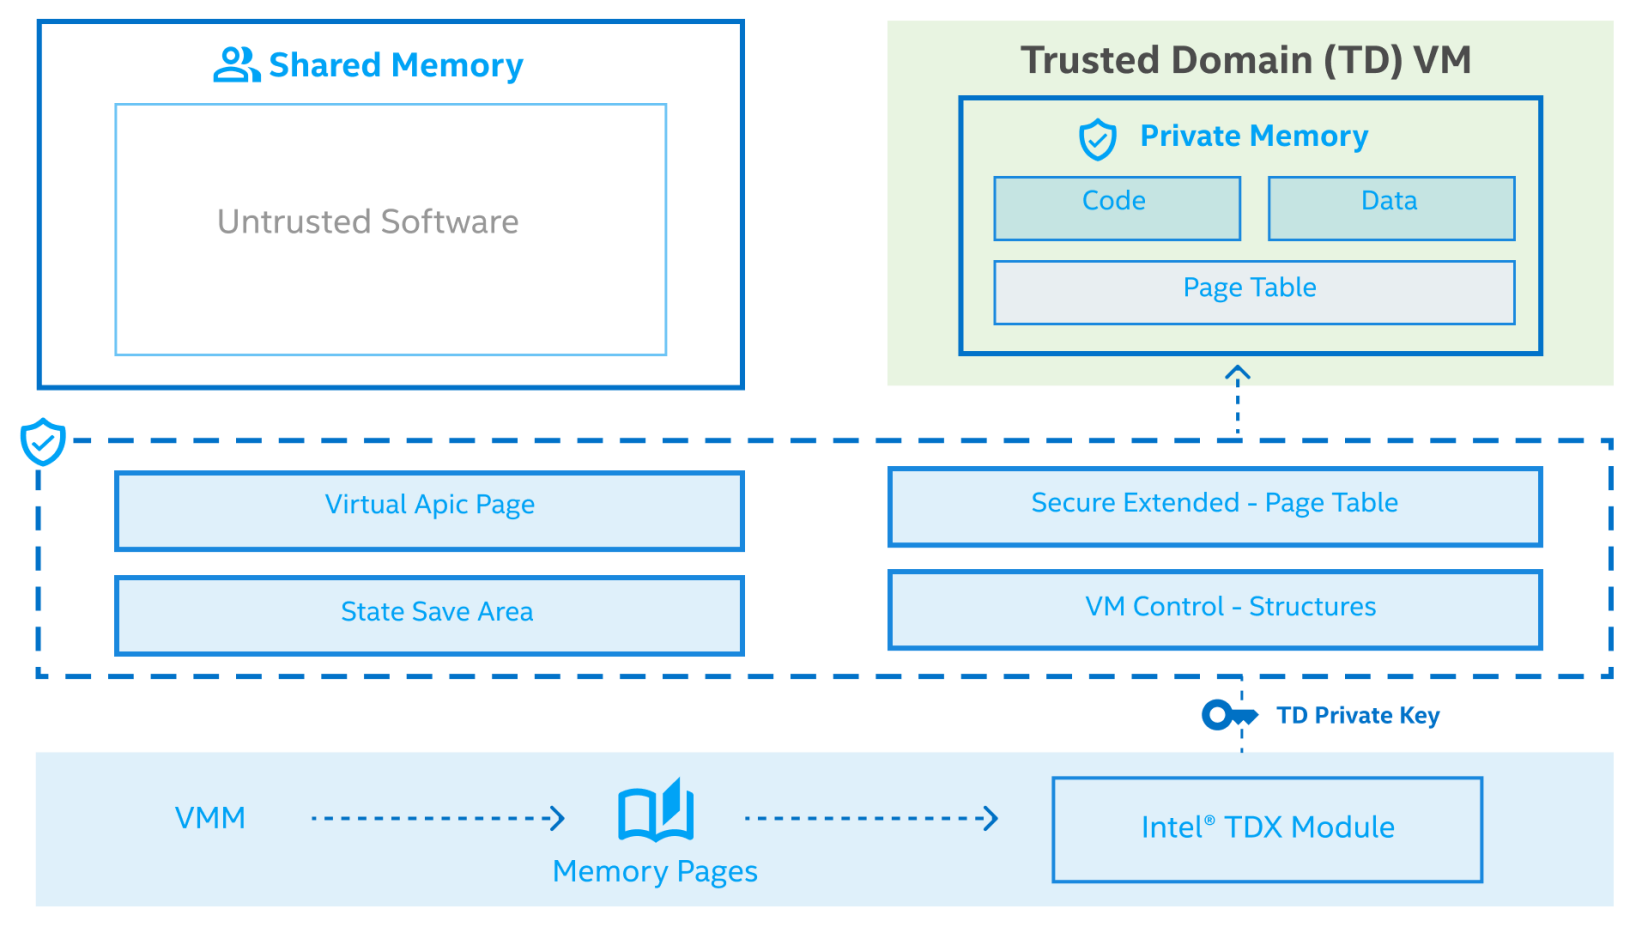
\includegraphics[width=0.6\textwidth]{tdx.png}
    \caption{Intel TDX Architecture}
    \label{fig:tdx}
\end{figure}

\begin{itemize}
    \item \textbf{IO virtualization.} It introduces a method for direct device assignment to TEEs without the need for shared buffers, enhancing both functionality and performance.

    \item \textbf{Security model.} The architecture ensures that only the TEE Device owner can decide which TEE-IO device interface is trustworthy, with strict access controls and data isolation.
    
    \item \textbf{Trusted execution.} Intel TDX Connect extends the TDX hardware with private MMIO and DMA access control, along with end-to-end data protection using PCIe selective IDE streams.
    
    \item \textbf{Architecture overview.} It provides a comprehensive framework for establishing trust between a TD (TEE Device) and a TDI (TEE Device Interface), securing the data path, and supporting the TDISP (TEE Device Interface Security Protocol) assignment and removal lifecycle.
\end{itemize}

\subsection{AMD SEV-SNP}

AMD SEV-SNP (Secure Encrypted Virtualization--Secure Nested Paging) \cite{snp} builds upon existing SEV and SEV-ES functionality while adding new hardware-based security 
protections. SEV-SNP adds strong memory integrity protection to help prevent malicious hypervisor-based attacks like data replay, memory re-mapping, and more in order to create an isolated execution 
environment. Also, SEV-SNP introduces several additional optional security enhancements designed to 
support additional VM use models, offer stronger protection around interrupt behavior, and offer 
increased protection against recently disclosed side channel attacks. The key features are as follows:

\begin{itemize}
    \item 
    \textbf{Memory integrity protection.} SEV-SNP enhances VM isolation by adding strong memory integrity protection to prevent malicious attacks like data replay and memory re-mapping.
    
    \item \textbf{Enhanced security features.} It offers optional protections against malicious interrupt injection, speculative side channel attacks, and rollback attacks on trusted computing base (TCB) components.
    
    \item \textbf{Flexible VM privilege levels.} The architecture introduces Virtual Machine Privilege Levels (VMPLs) that allow a VM to divide its address space into four hierarchical levels for additional security controls.
    
    \item \textbf{Advanced attestation and migration.} SEV-SNP supports flexible attestation, enabling VMs to request attestation reports at any time, and introduces an improved migration policy with the involvement of a Migration Agent (MA).
\end{itemize}

However, \citeauthor*{paradvzik2024formal} found attacks on several authentication and attestation properties, including \textbf{the compromise of attestation report integrity}. They also discover a vulnerability that \textbf{allows a cloud provider to trick a third party} into incorrectly believing that an SNP-protected guest is running on a platform with secure, up-to-date firmware. Slight modifications to the design which let third parties detect guest migrations to vulnerable platforms are proposed in \cite{paradvzik2024formal}.

\subsection{Arm CCA}

Arm proposed the design of Arm Confidential Compute
Architecture (CCA) \cite{cca} shown in Figure \ref{fig:cca} and its hardware security
primitive --- Realm Management Extensions (RME) --- to
support confidential computing in next-generation Arm
devices. CCA introduces \textbf{realms}, the basic unit of the confidential
computing environment, and the Realm Management
Monitor (RMM), which behaves as a thin hypervisor for
realm isolation. To mitigate the latency in realm execution,
an untrusted hypervisor is delegated to schedule the realms
and manage memory resources, but cannot access realms \cite{wang2024cage}.

\begin{figure}[h]
    \centering
    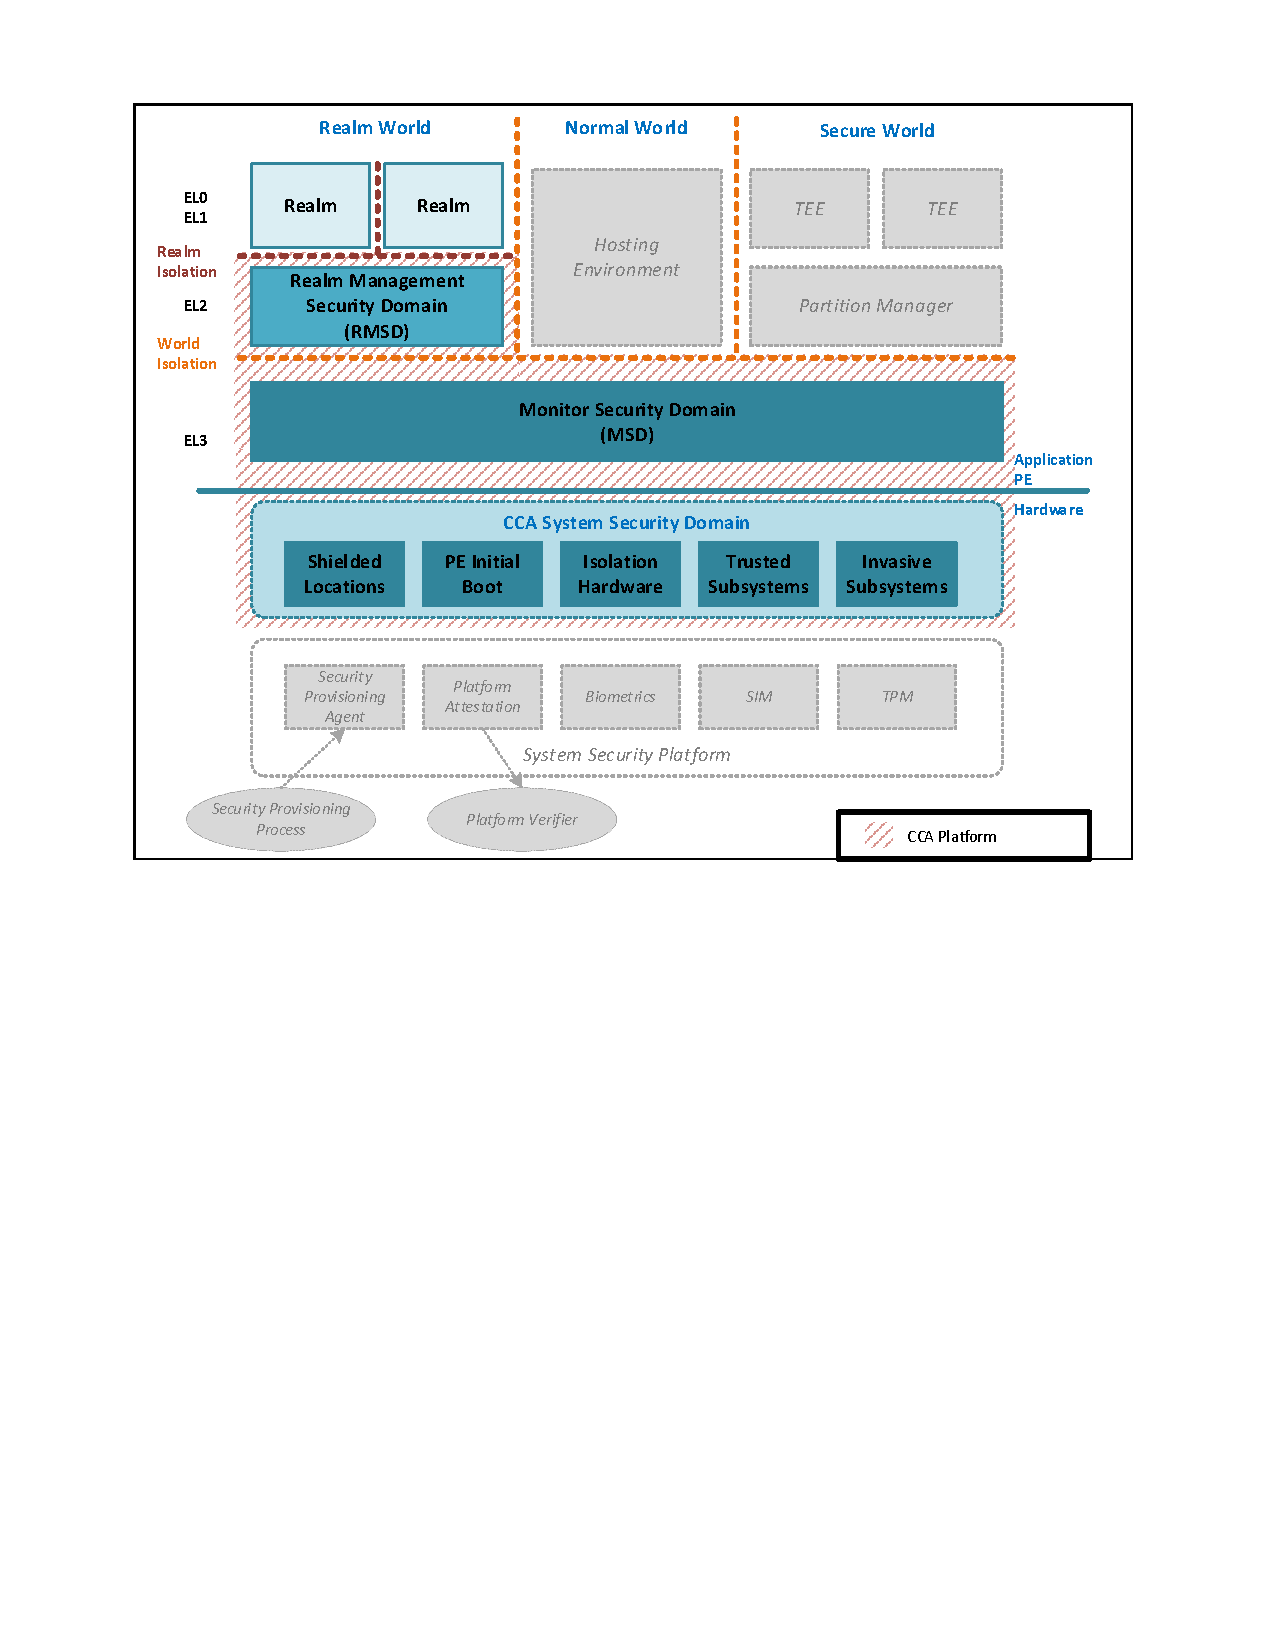
\includegraphics[width=0.7\textwidth]{cca.pdf}
    \caption{Elements of CCA \cite{armcca}}
    \label{fig:cca}
\end{figure}

\subsection{RISK-V: Penglai}

RISK-V-based Penglai \cite{penglai} is an open-source RISC-V enclave system using
a secure monitor to manage all the enclaves shown in Figure \ref{fig:penglai}. It first introduces two \textbf{new architectural
primitives}, Guarded Page Table (GPT) and Mountable
Merkle Tree (MMT): GPT protects page table pages and
enables memory isolation with page-level granularity, and
MMT is a new abstraction to achieve on-demand and scalable
memory encryption and integrity protection. Leveraging these
two primitives, a lightweight secure monitor running in the
most privileged mode is in charge of enclave management
and maintaining security guarantees. To mitigate the high
overhead of enclave creation due to costly secure memory initialization,
we propose a new type of enclave, called shadow
enclave, to support fork-style \textbf{fast enclave creation}.

\begin{figure}[h]
    \centering
    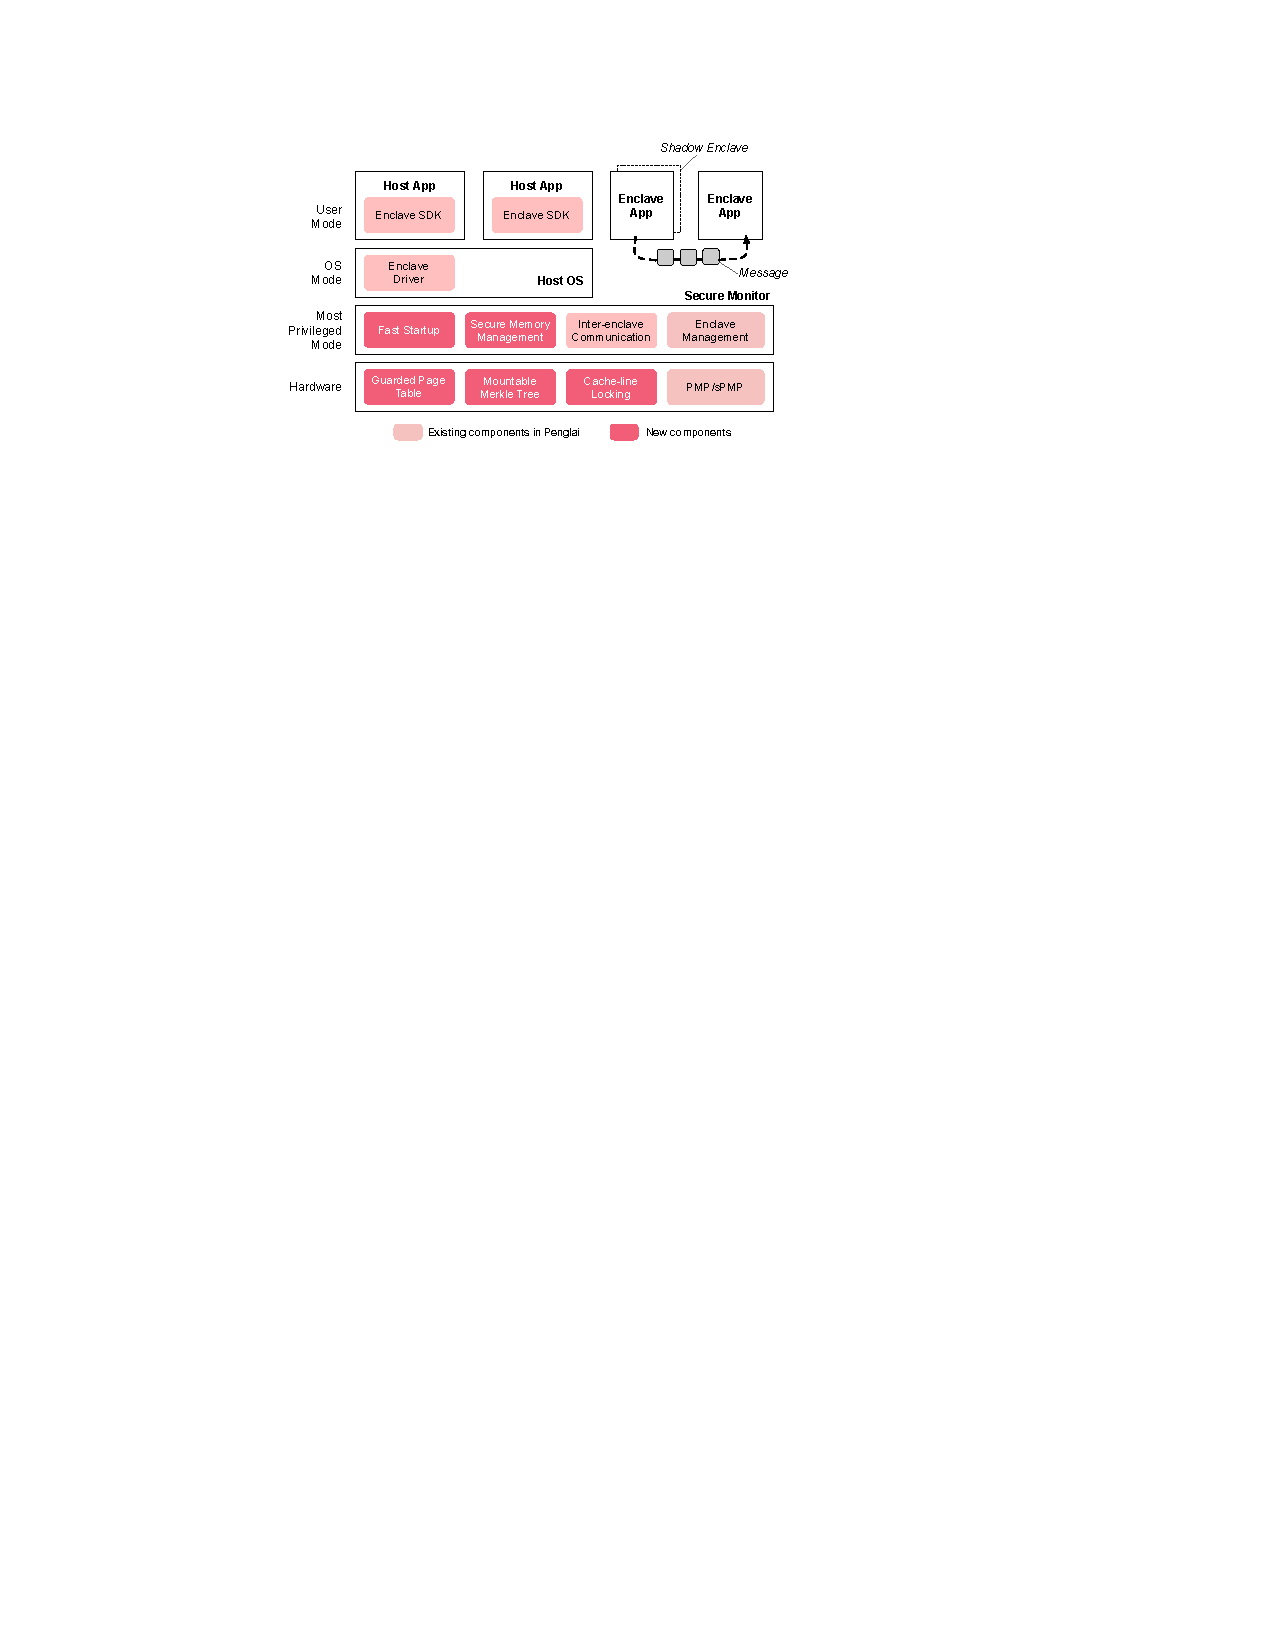
\includegraphics{penglai.pdf}
    \caption{Overview of Penglai Architecture}
    \label{fig:penglai}
\end{figure}

\section{Applications of TEE}

Use cases for TEEs start evolving in the areas of cloud computing,
blockchain, 
and artificial intelligence \cite{geppert2022trusted}. There are selected applications for each area: for cloud computing, Twilight for blockchain, PPFL for AI.

% \subsection{Cloud computing: VC3}

% \paragraph{Description.} VC3 (Verifiable Confidential Cloud Computing) \cite{vc3} is a TEE-based framework for secure distributed computation in the cloud. VC3 enables users to finish computations in the distributed
% MapReduce setting while maintaining the confidentiality of data and ensuring the accuracy and
% completeness of the final results.

\subsection{Cloud computing: Cyptomator}

With the evolution of computer systems, the amount
of sensitive data to be stored as well as the number of threats on
these data grow up, making the data confidentiality increasingly
important to computer users. Currently, with devices always
connected to the Internet, the use of cloud data storage services
has become practical and common, allowing quick access to
such data wherever the user is. Such practicality brings with
it a concern, precisely the confidentiality of the data which is
delivered to third parties for storage. In the home environment,
disk encryption tools have gained special attention from users,
being used on personal computers and also having native options
in some smartphone operating systems.

In \cite{closer20}, \citeauthor*{closer20} uses
the data sealing, feature provided by the Intel Software Guard
Extensions (Intel SGX) technology, for file encryption. A virtual
file system (\textbf{CryptoFS}) is created in which applications can store their data,
keeping the security guarantees provided by the Intel SGX
technology, before sending the data to a storage provider. This way,
even if the storage provider is compromised, the data are safe.
To validate the proposal, the \textbf{Cryptomator} software, which is a
free client-side encryption tool for cloud files, was integrated with
an Intel SGX application (enclave) for data sealing. The results
demonstrate that the solution is feasible, in terms of performance
and security, and can be expanded and refined for practical use
and integration with cloud synchronization services.

\begin{figure}[h]
    \centering
    \begin{minipage}[b]{.45\textwidth}
        \centering
        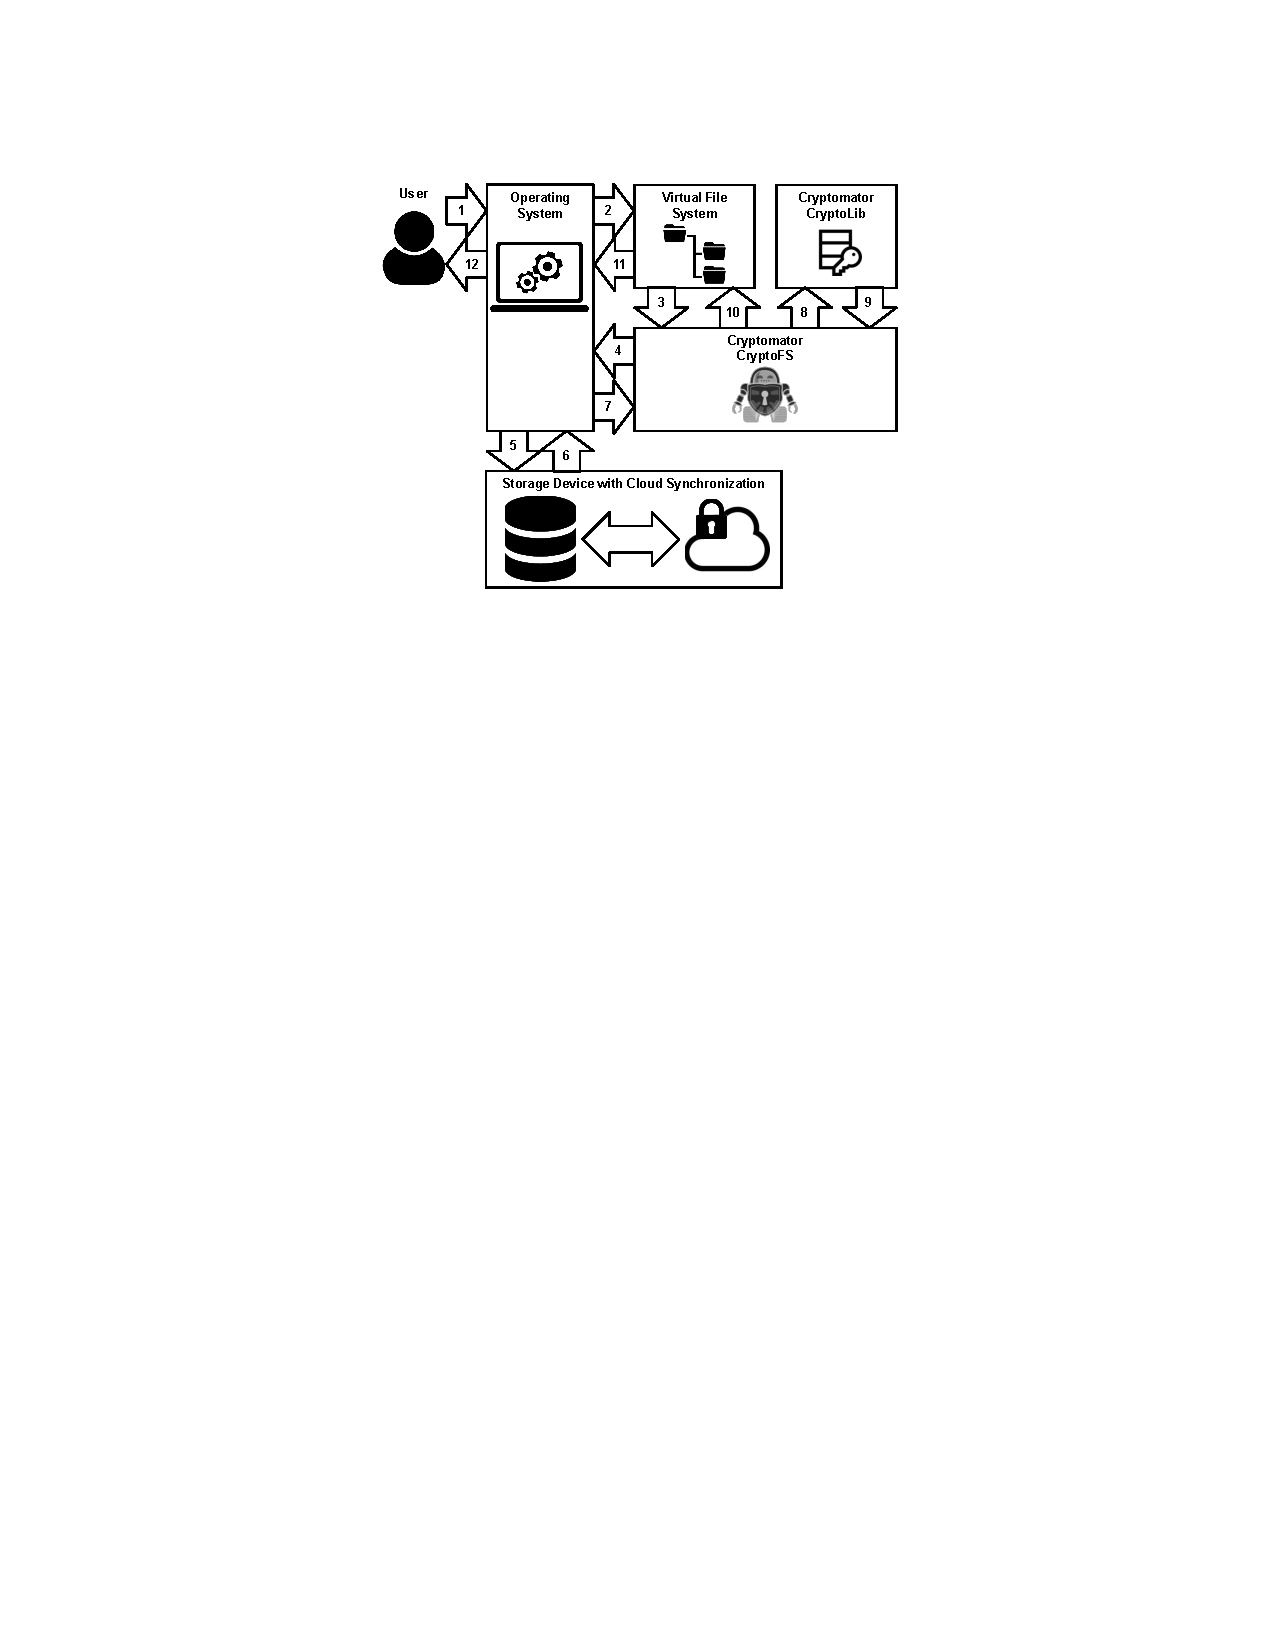
\includegraphics[width=\textwidth]{cyptomator.pdf}
        \caption{Workflow for reading and decrypting stored data with Cryptomator}
        \label{fig:cryptomator}
    \end{minipage}\hfill
    \begin{minipage}[b]{.45\textwidth}
        \centering
        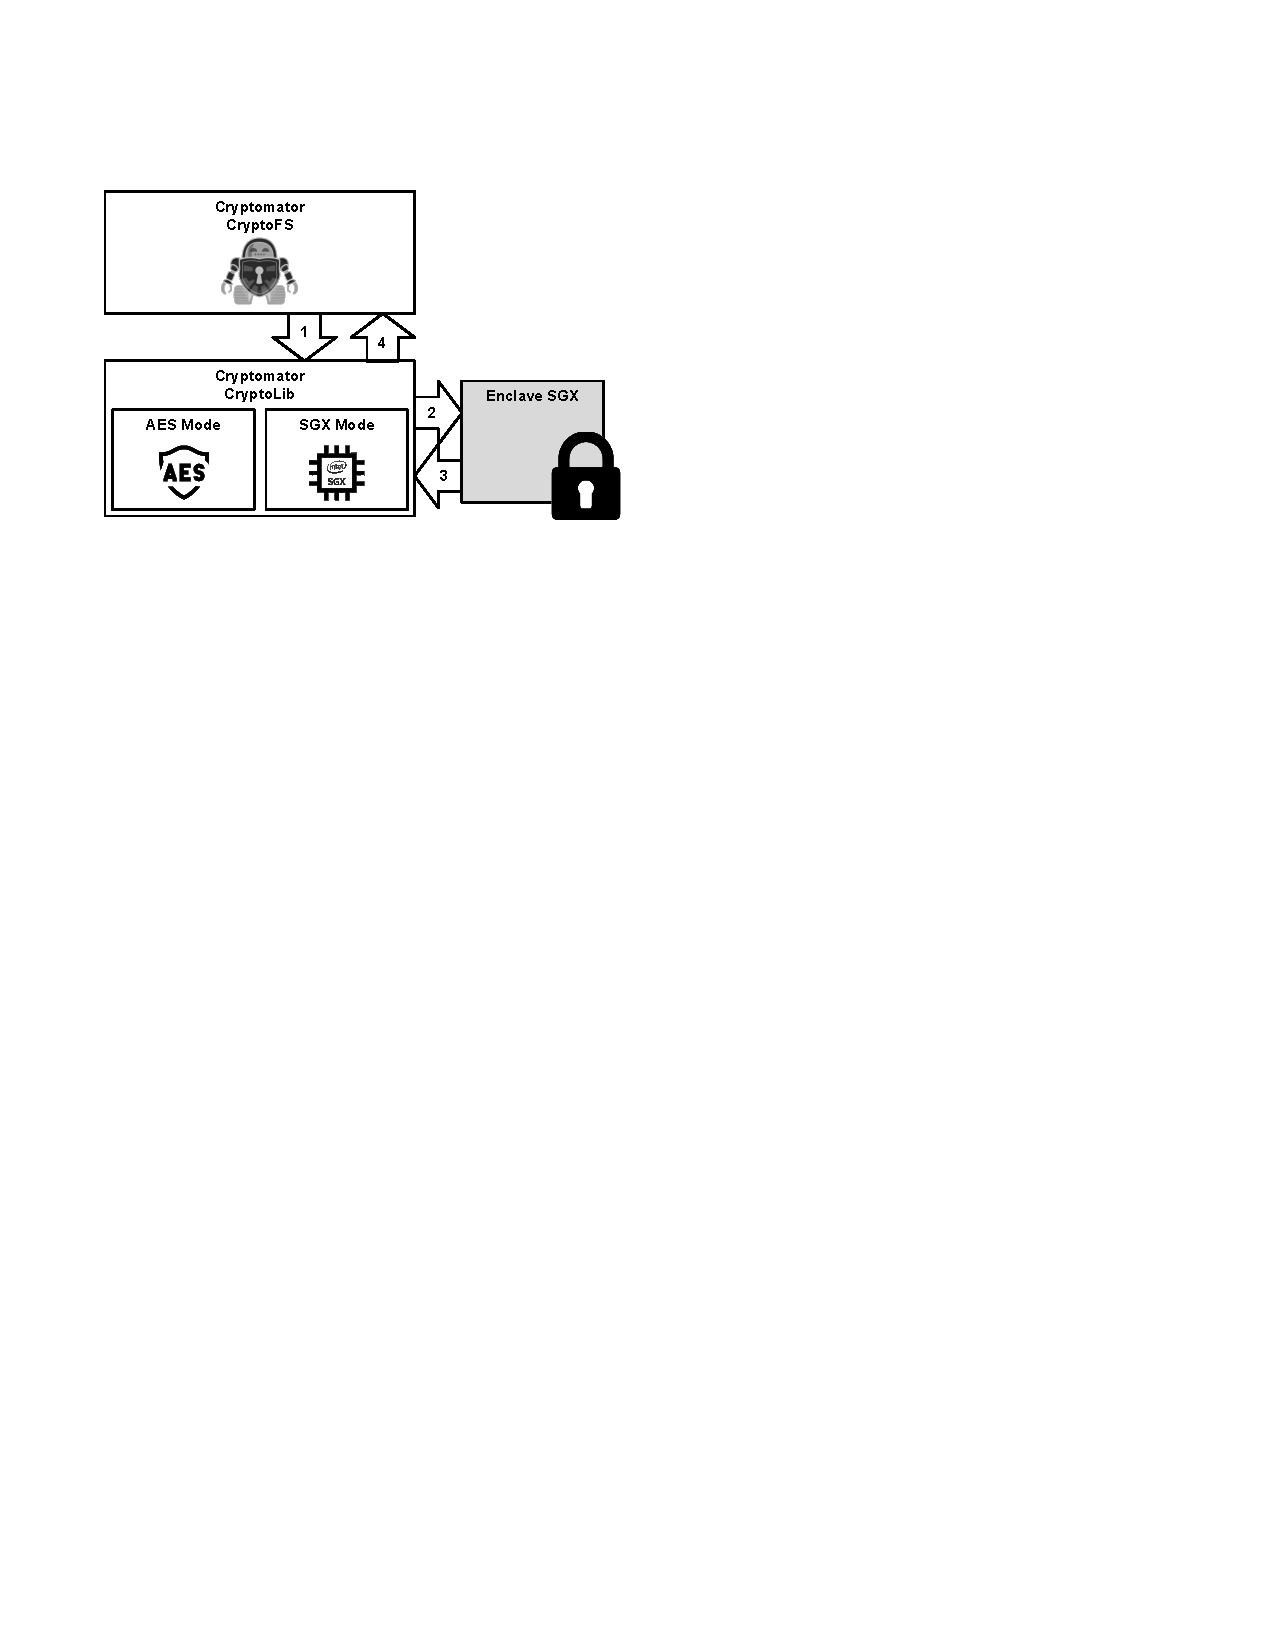
\includegraphics[width=\textwidth]{cyptofs.pdf}
        \caption{Workflow performed for data encryption and decryption through the Cryptomator}
        \label{fig:cryptofs}
    \end{minipage}
\end{figure}

The process of reading the files provided by the application
is shown in Fig \ref{fig:cryptomator}:
(1) The user requests the operating system to open a file;
(2) The operating system requests FUSE for file data. FUSE
allows the userspace applications export a filesystem
to the Linux kernel, with functions to mount the file
system, unmount it and communicate with kernel;
(3) FUSE forwards this request to the Cryptomator, using
the CryptoFS library;
(4) Cryptomator requests the operating system to have the
file data fetched from the storage device;
(5) The operating system locates the data;
(6) These data are loaded into the main memory;
(7) The operating system provides these data to the Cryptomator;
(8) The CryptoFS library sends the encrypted data to the
CryptoLib library;
(9) The CryptoLib library decrypts the received data and
returns them to CryptoFS library;
(10) The CryptoFS library sends the decrypted data to FUSE;
(11) FUSE forwards such data to the operating system;
(12) Finally, the operating system provides the user with the
decrypted file.

Fig \ref{fig:cryptofs} describes the process of sending and receiving data
between CryptoFS and CryptoLib libraries, which includes
two additional steps for communication between the CryptoLib
library and the SGX enclave. The shaded box indicates
a trusted execution environment (SGX in this case), where \textbf{the
key is manipulated} and \textbf{the data are encrypted and decrypted}.
The communication flow is explained below:
(1) CryptoFS library calls encrypt/decrypt functions in
CryptoLib library, which contains AES and SGX modes;
(2) In SGX mode, CryptoLib library creates an enclave
and sends to it each data block to perform the encrypt/
decrypt process;
(3) Encrypt/decrypt blocks are send back to CryptoLib;
(4) Encrypt/decrypt data forward to CryptoFS library.

\subsection{Blockchain: Twilight}

Payment channel networks (PCNs) provide a faster and
cheaper alternative to transactions recorded on the blockchain.
Clients can trustlessly establish payment channels with relays
by locking coins and then send signed payments that
shift coin balances over the network's channels. Although
payments are never published, anyone can track a client's
payment by monitoring changes in coin balances over the
network’s channels.

Twilight \cite{twilight} is the first
PCN that provides a \textbf{rigorous differential privacy guarantee} to
its users. Relays in Twilight run a noisy payment processing
mechanism that \textbf{hides the payments they carry}. This mechanism
increases the relay's cost, so Twilight \textbf{combats selfish
relays} that wish to avoid it using a TEE that ensures they follow its protocol. The TEE
\textbf{does not store the channel's state}, which minimizes the trusted
computing base. Crucially, Twilight ensures that even if a relay
breaks the TEE's security, it cannot break the integrity of
the PCN. \Citeauthor*{twilight} implement Twilight
using Intel's SGX framework and evaluate its performance
using relays deployed on two continents and show that a route
consisting of 4 relays handles 820 payments/sec.

In detail, protocol messages and relay-to-TEE interface are shown in Figure \ref{fig:twilight}.

\begin{figure}[h]
    \centering
    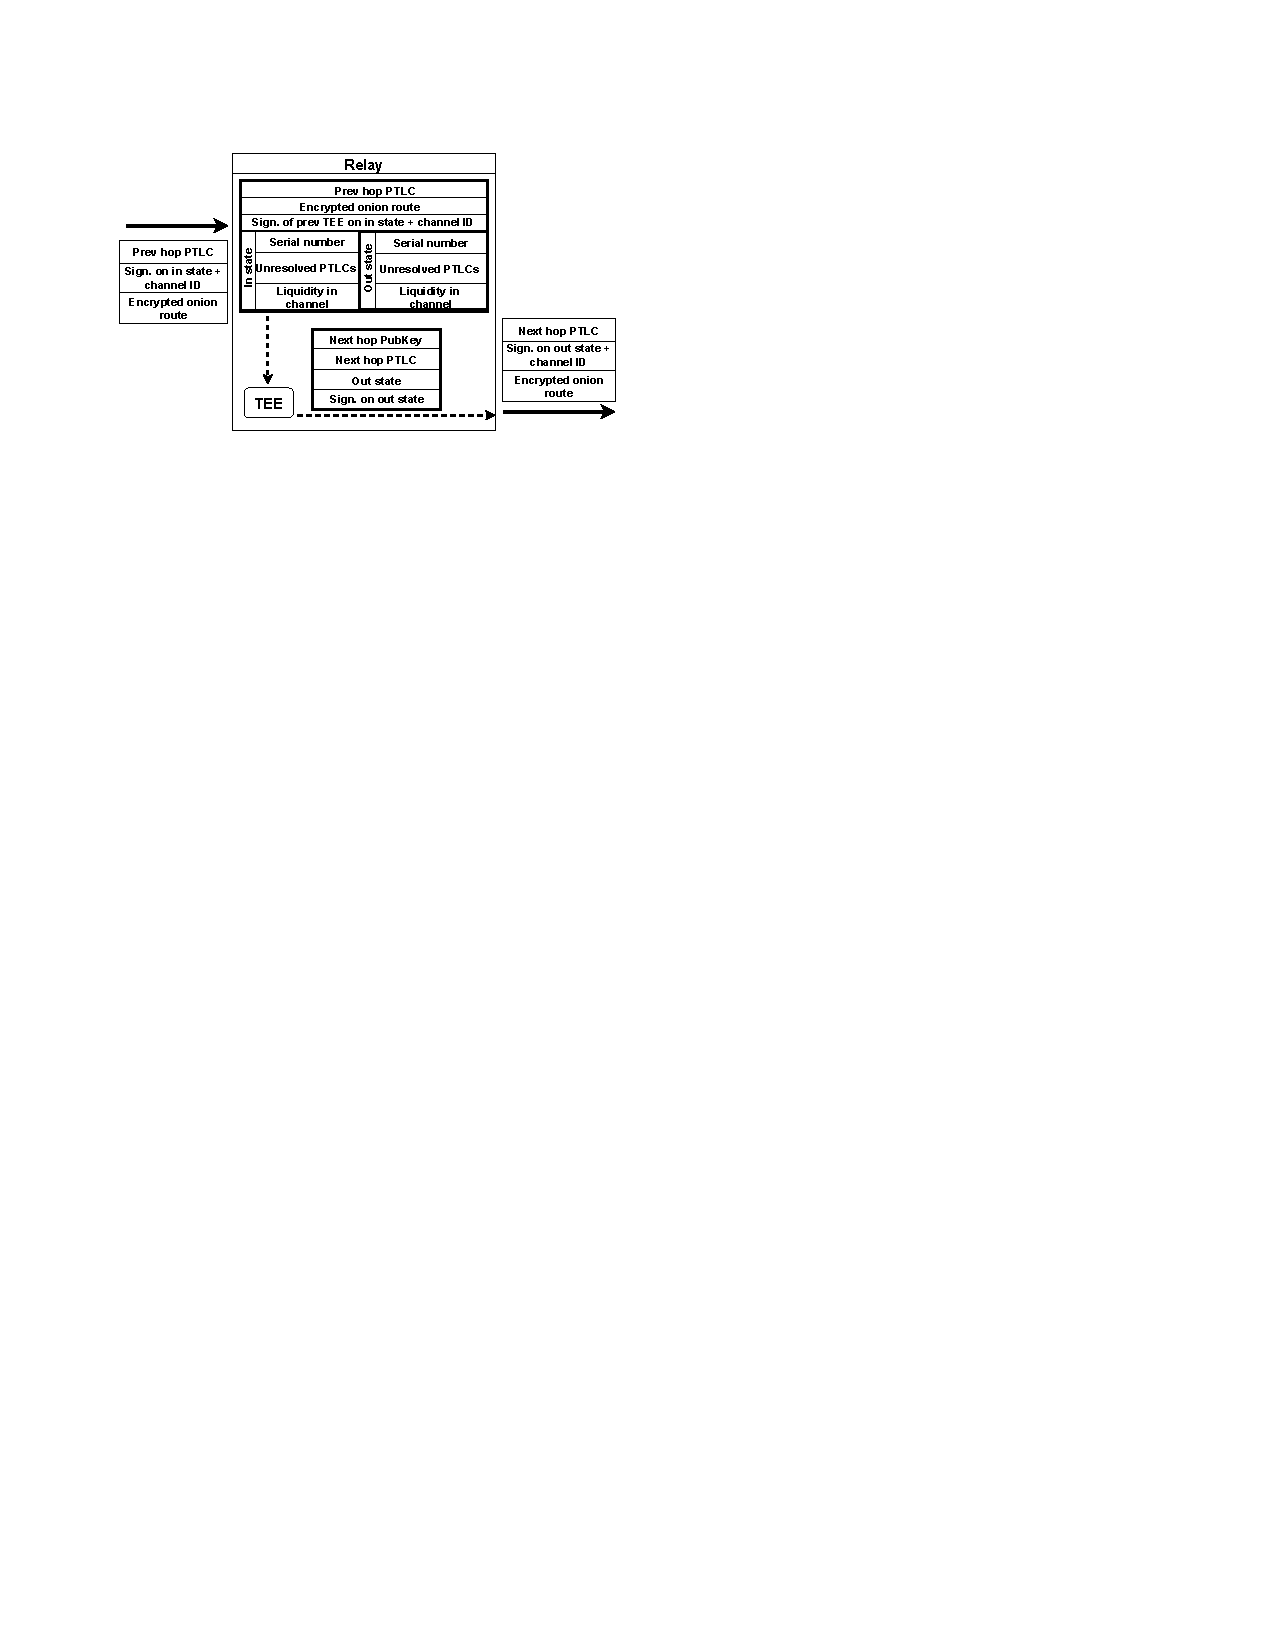
\includegraphics[width=0.8\textwidth]{twilight.pdf}
    \caption{Protocol messages and relay-to-TEE interface in Twilight}
    \label{fig:twilight}
\end{figure}

\paragraph{Establishing public keys and channel IDs.}

TEEs generate secret keys, and the corresponding public keys are bound to payment channels.
When a new payment channel is established, each party provides a public key to manage the account via a smart contract.
Clients can verify the payment processing logic within the TEE using remote attestation.
The smart contract's account address serves as the channel ID, ensuring that messages about the channel are unique and secure.

\paragraph{Processing payments inside TEEs.}

Relays receive and forward encrypted payments without knowing the outcome of the payment processing.
Payments are conditioned on a secret known only to the payee, using Private Time-Locked Contracts (PTLCs).
The TEE decides whether to approve a payment based on the current balance and pending payments, without storing the channel's state.
Payments are encrypted for the next TEE in the route, preventing relays from adjusting the noise distribution to the payment.

\paragraph{Channel teardown.}

Channels close by posting a transaction to the blockchain, splitting the locked coins between the channel endpoints.
Parties exchange signed closing balance messages after each payment, which are authorized by the TEE's secret key.
The smart contract allows for an appeal period where parties can dispute the closing balance with higher serial number messages.
Twilight can operate over blockchains that support private transactions, hiding the channel's closing balance split.

% Figure \ref{fig:twilight} illustrates
% how a relay interacts with its TEE. The enclave running
% inside the TEE does not store the channel's state but receives
% it from the relay with every payment processing request to
% decide whether to approve a payment.

% force relays to use TEEs. TEEs are isolated hardware that gives us the confidentiality and integrity, which means that the relay cannot change the code that runs inside TEE, see the memory or see which flow of the execution has occurred.

\subsection{AI: PPFL}

PPFL (Privacy-preserving Federated Learning with TEE) \cite{mo2021ppfl} is a framework for mobile systems to limit privacy leakages
in federated learning. It utilizes TEEs on clients for local training, and on servers
for secure aggregation, so that model/gradient updates are hidden
from adversaries. Figure \ref{fig:ppfl} provides an overview of the framework and the various
steps of the \textbf{greedy layer-wise training and aggregation}, which allows clients to collaboratively train a DNN model while
keeping the model's layers \textbf{always inside TEEs during training}. In general,
starting from the first layer, each layer is trained until convergence,
before moving to the next layer. In this way, PPFL aims to achieve
full privacy preservation without significantly increasing system
costs.

\begin{figure}[h]
    \centering
    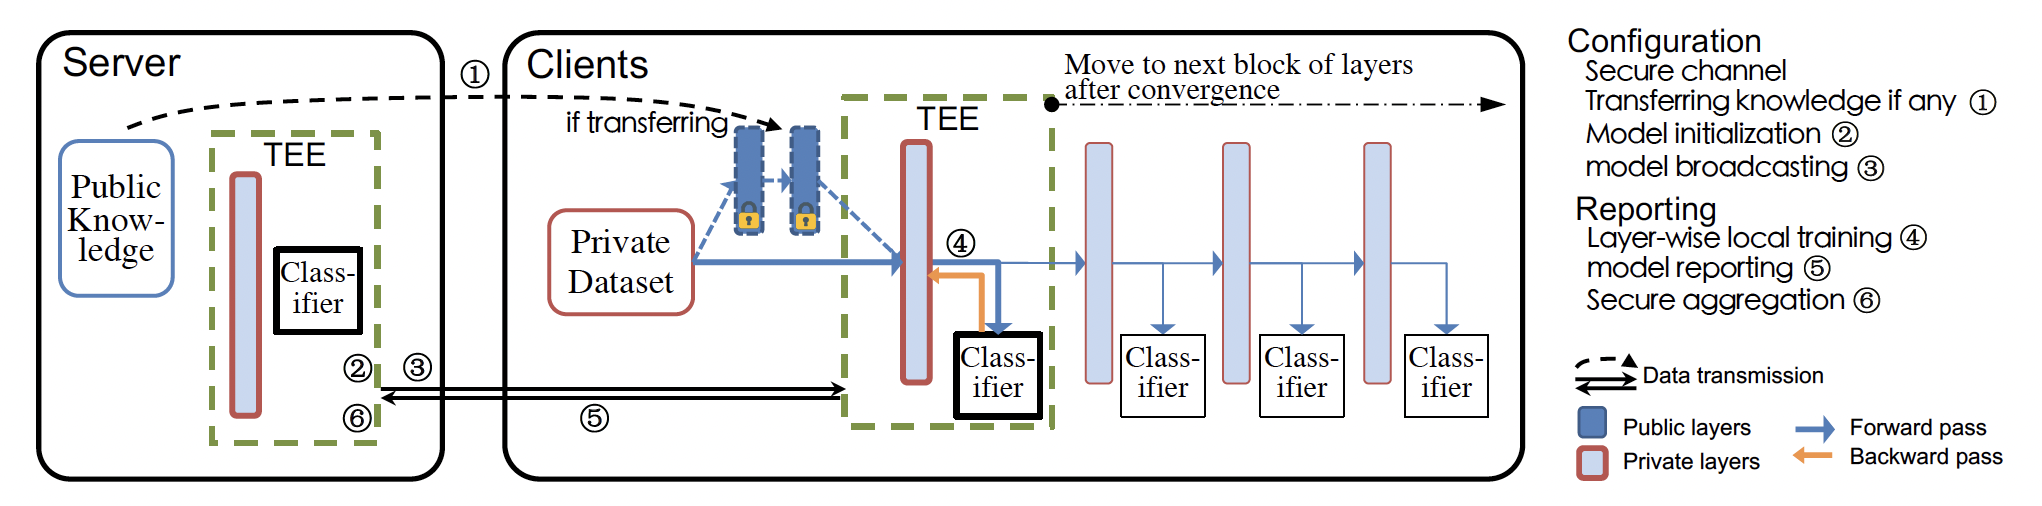
\includegraphics[width=\textwidth]{ppfl.png}
    \caption{A schematic diagram of the PPFL framework}
    \label{fig:ppfl}
\end{figure}

The brief process is as follows: In PPFL, the server can learn from public models. Thus, during
initialization, the server first chooses a model pre-trained on public
data that has a similar distribution with private data. The server
keeps the first layers, removes the last layer(s), and assembles new
layer(s) atop the reserved first ones. These \textbf{first layers} are transferred
to clients and are always kept frozen (step \circlednumber{1}). The server configures
the model architecture, decides the layers to be protected by TEEs,
and then \textbf{initializes model parameters} inside the TEE (step \circlednumber{2}). The latter ensures clients' local training starts with the same weight
distribution. In addition, the server \textbf{configures other training
hyper-parameters} such as learning rate, batch size, and epochs,
before transmitting such settings to the clients (step \circlednumber{3}). After model transmission and configuration using
secure channels, each client starts \textbf{local training} on their data on
each layer via a model partitioned execution technique (step \circlednumber{4}). Once local training of a layer is
completed inside TEEs, all participating clients \textbf{report the layer
parameters} to the server through secure channels (step \circlednumber{5}).
Finally, the server securely \textbf{aggregates the received parameters}
within its TEE and applies FedAvg, resulting in a new global
model layer (step \circlednumber{6}).

\section{Vulnerabilities of TEE}

Despite its appealing features, TEE is also vulnerable to several attacks, and
the survey in \cite{fei2021security} discusses these attacks in detail. There are two major attacks
that would affect secure computation: side-channel attacks and rewind attacks.

\subsection{Side channel attacks}

First, TEE may suffer from side-channel attacks which could
breach data privacy. They are mainly from timing, memory, and network side channels.

\paragraph{Timing side channel \cite{gupta2016using}.} Given different inputs, the running time of the program in the
enclave may be different too. By \textbf{monitoring the difference over the execution time}, an
attacker may derive some sensitive information about the input, e.g., a secret value reflecting
how many times a loop is executed. To solve this problem, one approach is to ensure the
program loaded into the enclave \textbf{always takes approximately the same amount of execution
time}.

\paragraph{Memory side channel \cite{sasy2017zerotrace}.} In some programs, \textbf{the access pattern} to the non-PRM memory
\textbf{may depend on the enclave's secret}. For example, if the enclave runs a binary search program,
the access pattern is a path from the root node to a leaf node, which may reveal the real
secret. Therefore the loaded program should \textbf{remove any correlation} between the memory
access pattern and the insider secret.

\paragraph{Network side channel \cite{zheng2017opaque}.} In a distributed system, \textbf{network access patterns} (e.g., sorting or
hash partitioning) may reveal sensitive information. Therefore, the network access protocol
should also be well-designed such that no sensitive information can be deduced from the
patterns.

\subsection{Rewind attacks}

TEEs may also be vulnerable to rewind attacks (or replay attacks), which allows an
attacker to actively \textbf{reset the state of the computation} \cite{bellare2001identification}. Note that such attacks may result in
catastrophic consequences for stateful computation, such as limited-attempt password checking. We cannot always expect the TEE to maintain the state securely for two reasons: (1) TEE
may be stateless in practice; (2) even for stateful TEE, the limited protected memory makes it fail
to correctly maintain a large state. Therefore, the designer should be careful and provides special
mechanisms to counter rewind attacks.

\printbibliography

\end{document}